\chapter{Guidance \& Navigation}
\label{chapter: guidance and navigation}


\section{Tasks and goals}
\label{sec: tasks and goals}
Classically, the Guidance \& Navigation subsystem handles locating the spacecraft in 3D space, tracks the position history, predicts and plans trajectory, and computes commands for the propulsion subsystem required to maintain the trajectory. The GNS must provide this functionality starting at separation from the cruise stage and ending at atmospheric entry. During the entry, navigation subsystem keeps track of position, altitude, velocity, and provides this information to the deployment subsystem to stage the entry procedures.

For the nominal VISTA mission, the task fundamentally boils down just to position tracking. Active control of horizontal position would require countering the winds, which at 55 km altitude reach up to 60 m/s.

Since the balloon follows with winds that reach up to 60 m/s (at 55 km altitude), active position control in the horizontal direction is unfeasible. Altitude control through the buoyancy/weight balance is possible, and necessary to allow for conducting scientific investigation at different altitudes or to counter disturbance from vertical winds (up to a few meters per second).

\section{Design options}
\label{sec: design options}

The main challenge of navigating around Venus is the scarcity of absolute position measurements. Since the thick cloud layer completely diffuses incoming sunlight and Venus doesn't have an intrinsic magnetic field, the only available references are the Venusian surface and telecommunications with orbiters or Earth.

\begin{figure}[H]
    \centering
    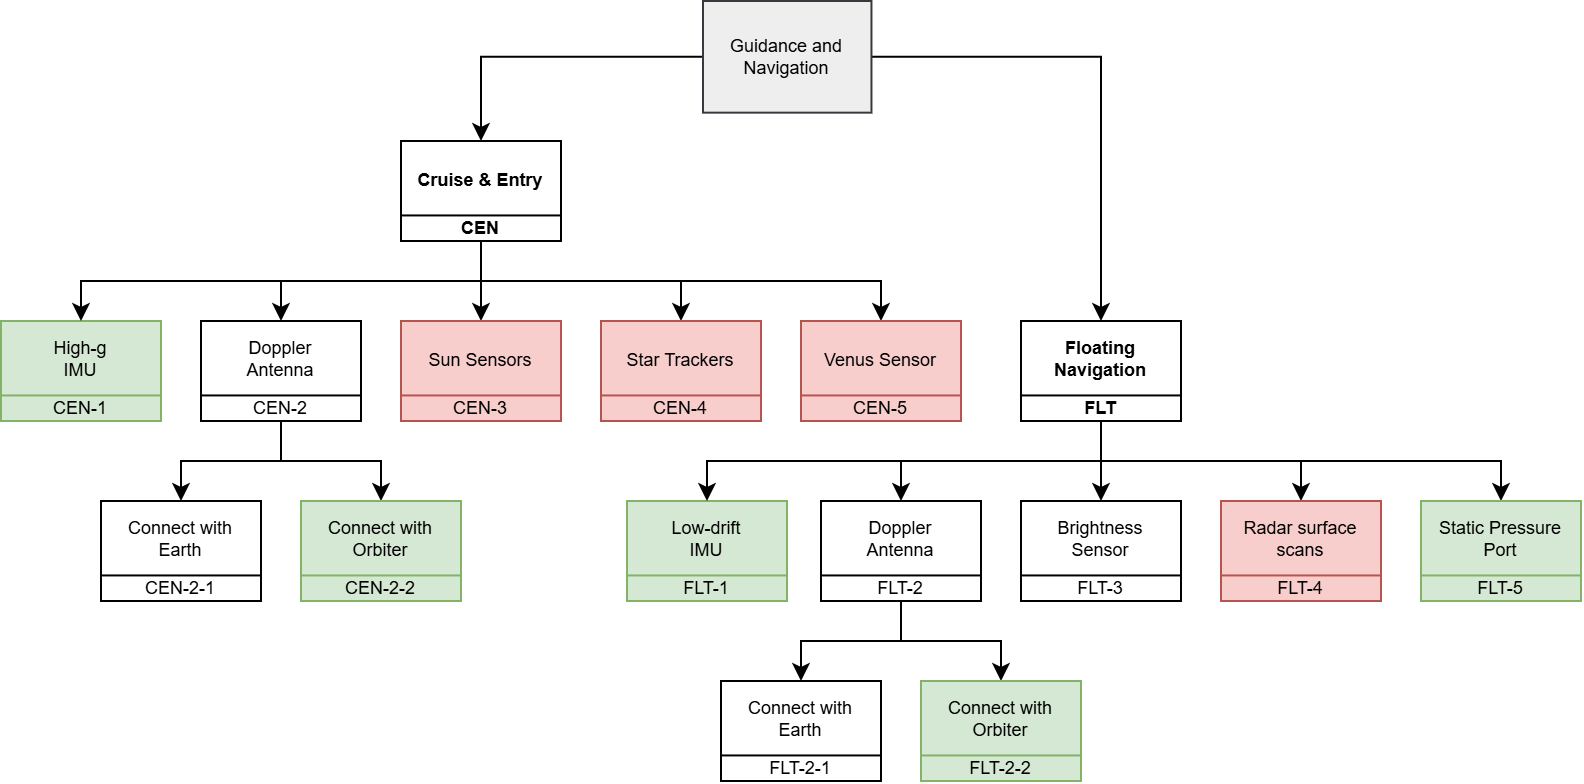
\includegraphics[width=\linewidth]{fig/DOT_navigation.png}
    \caption{Design Option Tree of the Guidance \& Navigation Subsystem}
    \label{fig: dot navigation}
\end{figure}

For the cruise and entry stage, the selected methods of navigation include Doppler antenna tracking with respect to the orbiter and propagation with a high-g inertial measurement unit. Conventional spacecraft strategies like sun senors or star trackers are not selected, since they involve dedicated equipment that only needs to operate for a few hours and is later discarded, which is very cost and mass inefficient.

During the nominal mission, balloon altitude can be easily determined by using a static pressure port and comparing to the reference atmosphere. In case no barometers are available in payload, a dedicated one will be necessary. The two methods of absolute determination of geographic coordinates are Doppler antenna tracking and radar surface imaging. Radar imaging is deemed unfeasible to due great mass and power requirements. Doppler tracking is designed to operate between the balloon and the relay orbiter. While tracking directly from Earth is possible, and has been done for the Vega missions, it would require dedicated time of the deep-space communication network, provides very poor data rates and only works for half the time due to Venus occlusion. It is not considered for nominal operation.

Since active control of the aerobot's geographic coordinates is not considered, real-time knowledge of position isn't critically necessary. Inertial measurements of the path can provide a convenient position estimation at times when the communication with the orbiter is not available, but are limited by the drift rate of the inertial sensors. Post-facto knowledge of absolute position and attitude measurements is a far easier task. As shown by \cite{Frazier2022}, the drift errors of the IMUs can be anchored at the beginning and end of the communications blackout period, which effectively halves the total drift period.  

\begin{figure}[H]
    \centering
    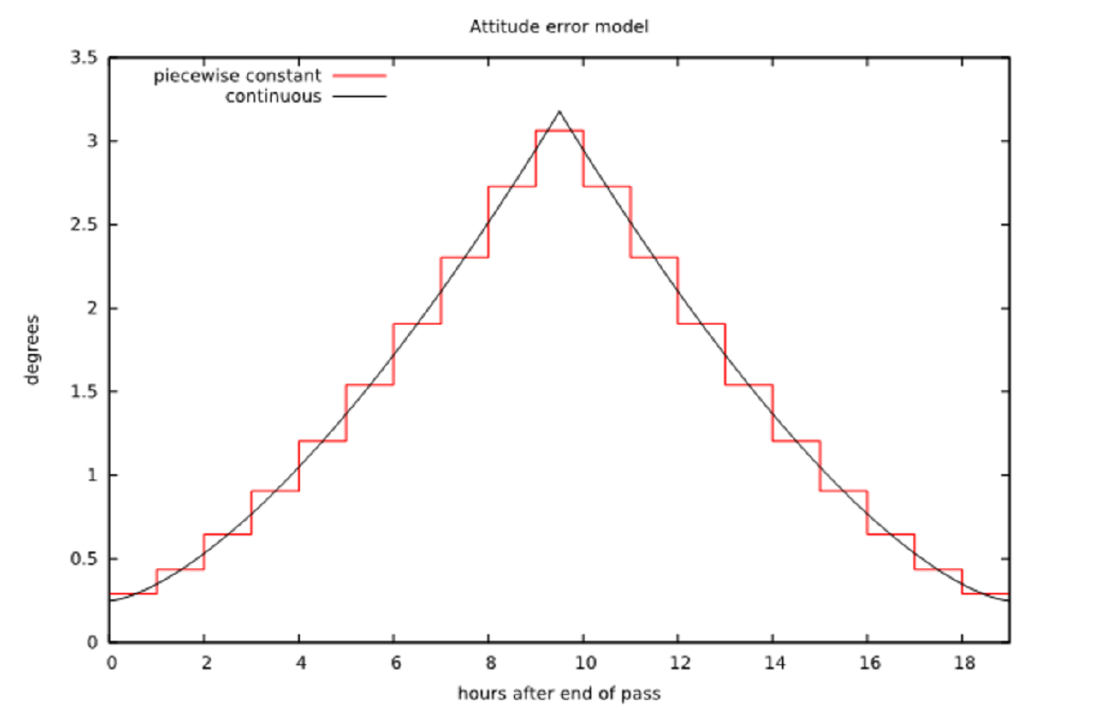
\includegraphics[width=0.75\linewidth]{fig/IMU_drift.png}
    \caption{Attitude error modeling during a tracking gap \cite{Frazier2022}}
    \label{fig: imu drift}
\end{figure}

\section{Hardware components}
\label{sec: hardware components}

The navigation subsystem is a bit unique, in a sense it is primarily software-based, and all hardware required by it is used by other subsystems. The main purpose of the antenna used for Doppler tracking is as a communications relay, the IMUs are mostly considered for ADCS, and the barometers are part of payload. The mass and power of these elements is included in the budgets of the corresponding subsystems. For convenience, it is also summarized in \autoref{tab: navigation hardware components} below. Notice that when operating, the IMUs necessarily require a 100\% duty cycle. A break in IMU tracking would introduce unknown and indeterminable deviations and make path reconstruction impossible. The pressure probe can have a very slow duty cycle. Brief measurements a few times per minute should be enough for good altitude tracking, since the balloon system altitude change is comparatively quite slow. It is important to have a data source acting as the official arbiter of daytime/nighttime determination. This can potentially be inferred from the working of the solar panels, or from payload instruments like a nephelometer or a camera. If such functionality cannot be easily and reliably provided by other subsystems, a dedicated ambient light intensity sensor should be installed.


\begin{table}[H]
\centering
\caption{Guidance \& Navigation Subsystem Components}
\label{tab: navigation hardware components}
\resizebox{\textwidth}{!}{%
\begin{tabular}{llllll}
\hline
\textbf{Component} &
  \textbf{Example Model} &
  \textbf{Power {[}W{]}} &
  \textbf{Duty Cycle {[}\%{]}} &
  \textbf{Mass {[}kg{]}} &
  \textbf{Avg. Power {[}W{]}}\\ \hline
Communications Antenna  & See Communications Subsystem      & 8              & 25\%                                       & \textless{}0.300 & 2       \\
High-g IMU              & GuideNav GUIDE 600G               & 2 (estimated)  & 100\% (cruise and entry only)              & 0.050            & 2       \\
Low-drift accelerometer & 3 x Honeywell single axis QA-3000 & 1.5            & 100\%                                      & 0.210            & 1.5     \\
Low-drift gyroscope     & Safran STIM300                    & 1.5            & 100\%                                      & 0.055            & 1.5     \\
Static Pressure Probe   & See Payload                       & \textless{}0.1 & 10\%                                       & \textless{}0.010 & $\sim$0 \\ \hline
                        &                                   &                & \textbf{Total}                             & $\sim$0.425      & 7      
\end{tabular}%
}
\end{table}

\section{Software components}
\label{software components}

During nominal operation, the Guidance and Navigation subsystem has two primary operational tasks: acquiring and storing tracking data from on-board sensors (\autoref{fig: nav flow 1}), and using the Doppler effects of the radio connection with the antenna to estimate absolute location and attitude (\autoref{fig: nav flow 2}). The GNS also cooperates with the buoyancy and nitrogen extraction subsystem to monitor and control the aerobot altitude (\autoref{fig: nav flow 3}).

\begin{figure}[H]
    \centering
    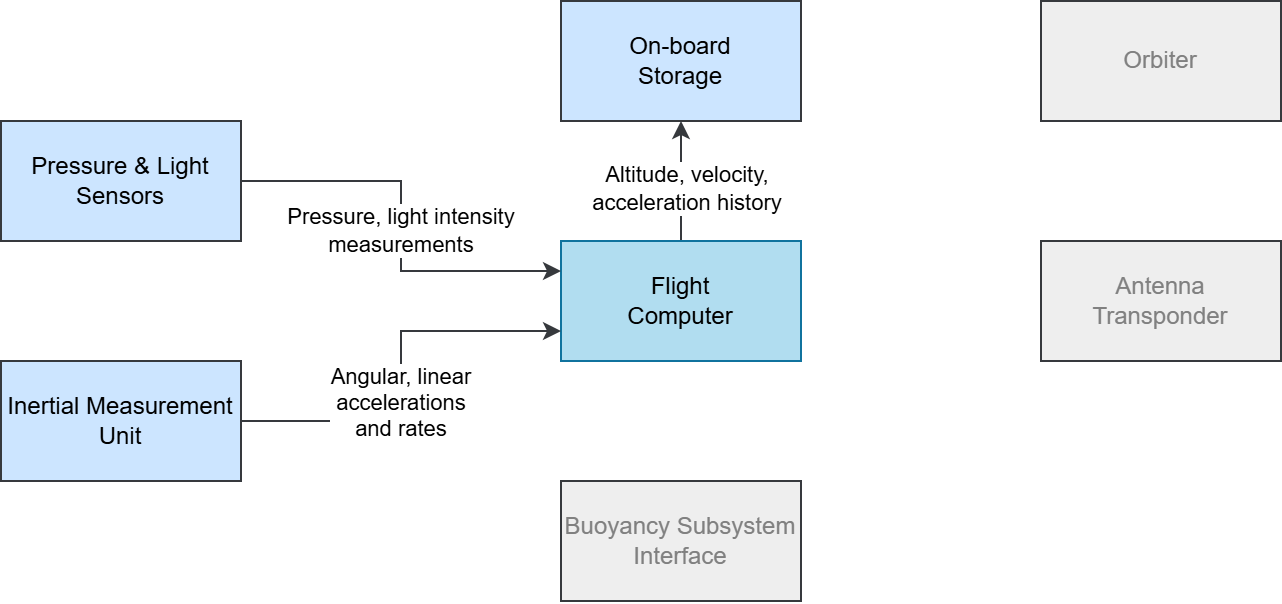
\includegraphics[width=0.85\linewidth]{fig/navigation_flow_1.png}
    \caption{GNS data flow of measurement acquisition}
    \label{fig: nav flow 1}
\end{figure}

During measurement acquisition, which keeps occurring throughout the nominal mission, the flight computer periodically samples the static pressure sensor (and the ambient light intensity sensor, if available). The inertial measurement unit runs continuously. The information about position and accelerations is logged and stored as telemetry for later use.

\begin{figure}[H]
    \centering
    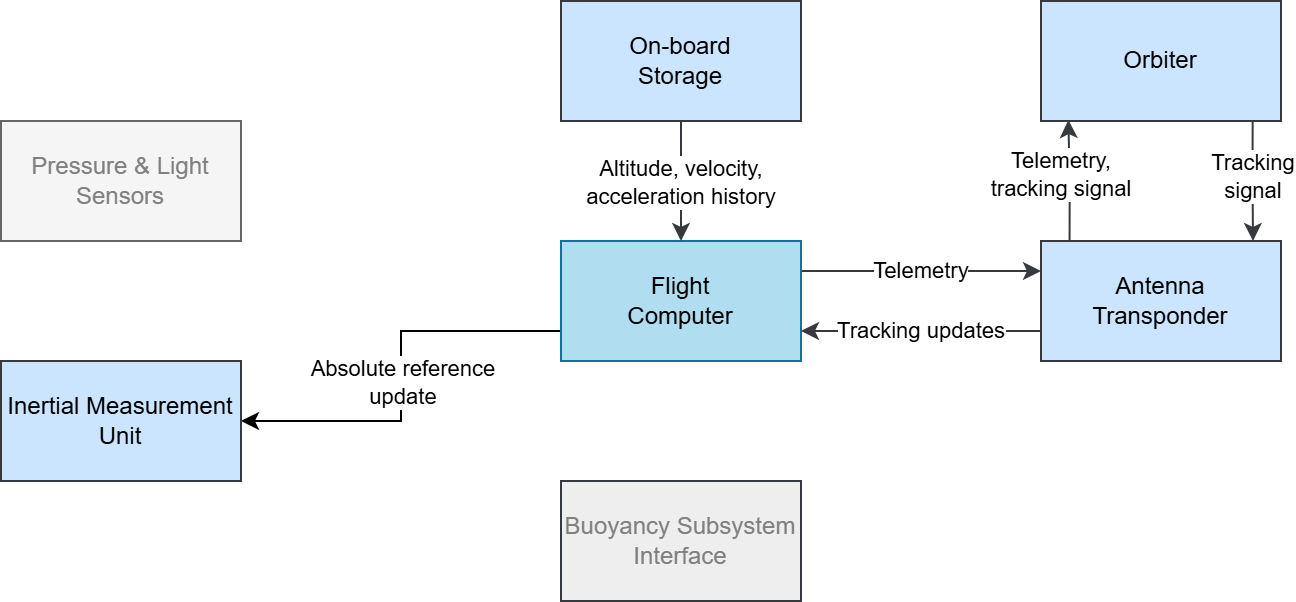
\includegraphics[width=0.85\linewidth]{fig/navigation_flow_2.png}
    \caption{GNS data flow during active Doppler ranging}
    \label{fig: nav flow 2}
\end{figure}

Active Doppler ranging is an operation mode that can only be active when the communication window to the orbiter is open and there is sufficient power available (it might be unfeasible to run this mode at night). During the transmission of standard telemetry or scientific data, the exact signal signature is studied to determine the distance between the aerobot and the orbiter (range), as well as the velocity and attitude change of the aerobot (range rate). If necessary for the procedure, a dedicated tracking signal will be transmitted instead. Using the tracking data, the absolute reference for the IMU can be updated.

\begin{figure}[H]
    \centering
    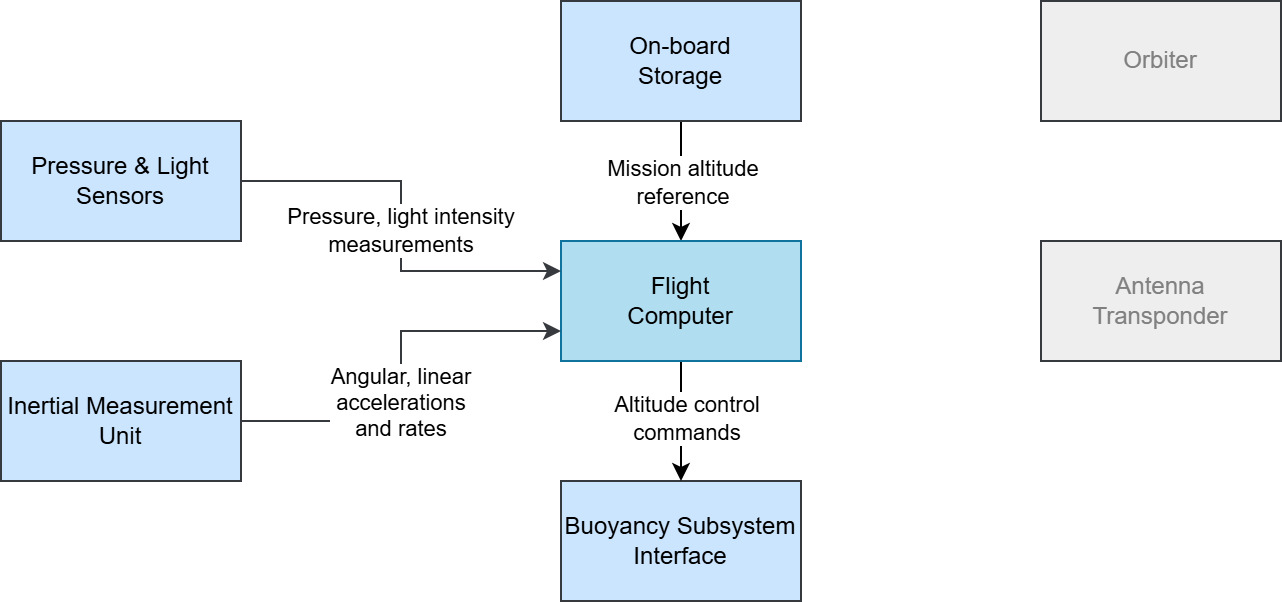
\includegraphics[width=0.85\linewidth]{fig/navigation_flow_3.png}
    \caption{GNS data flow during altitude control}
    \label{fig: nav flow 3}
\end{figure}

The GNS monitors and controls altitude continuously. The measured state is compared to a reference derived based on scientific targets and mission planning. The altitude control command is computed and sent to the buoyancy subsystem. The exact abstraction level of the navigation controller interface with the buoyancy subsystem code is undecided at this stage. A promising design for a model predictive altitude controller is given in \cite{apostol2025}, and is based on sequential convex programming for repeatedly approximating nonlinear aerobot dynamics.

\section{Navigation Verification and Validation}
The VISTA Mission would be the first one to deploy a Venus aerobot with long-term tracking abilities and altitude control. Its navigation subsystem mostly relies on software procedures and interacts with large scale Venusian weather, which is largely not understood. As such, conclusively proving accurate and reliable functioning is not feasible. Verification and validation efforts should focus on general robustness and ability to retain some functionality in many environments.

Extensive software verification shall be conducted to guarantee internal consistency and predictability. The behaviour of the navigation subsystem shall be investigated through simulation using atmospheric models (e.g. the Venus Climate Database \cite{VenusClimateDatabase}). Given the mission timeline, it should be possible to develop a dedicated climate model designed specifically for aerobot position propagation. The simulations should encompass a wide range of atmosphere input variables, to hopefully contain within itself the actual conditions that will be encountered durin the nominal mission.

